\chapter{Conception fonctionnelle et technique}

\textbf{Ma démarche de conception :} J'ai suivi une approche itérative : je modélise d'abord pour clarifier mes idées, je valide avec des utilisateurs, puis j'implémente. Cette méthode garantit que je réponds aux vrais besoins des joueurs.

\section{Les cas d'usage (Use Cases)}

Avant la première ligne de code, j'ai listé toutes les interactions possibles avec l'application.

\subsection{Les acteurs du système}

\begin{itemize}
    \item \textbf{Joueur débutant :} Veut apprendre les raids et trouver une équipe bienveillante
    \item \textbf{Joueur expérimenté :} Veut organiser ses sessions rapidement
    \item \textbf{Leader d'escouade :} Gère une équipe et suit la progression
    \item \textbf{Administrateur :} Modère les contenus
    \item \textbf{Système Bungie (API) :} Fournit les données de jeu
\end{itemize}

\subsection{Les cas d'usage principaux}

\begin{itemize}
    \item \textbf{UC001 :} Se connecter avec son compte Bungie
    \item \textbf{UC002 :} Consulter un guide de raid interactif
    \item \textbf{UC003 :} Créer et gérer une escouade
    \item \textbf{UC004 :} Planifier une session de raid
    \item \textbf{UC005 :} Gagner et consulter des badges
    \item \textbf{UC006 :} Synchroniser ses données de jeu
\end{itemize}

\subsection{Exemple détaillé : Consultation d'un guide}

\textbf{Acteur :} Joueur connecté \\
\textbf{Déclencheur :} Il veut apprendre un raid \\
\textbf{Scénario nominal :}
\begin{enumerate}
    \item Il choisit un raid dans la liste
    \item La plateforme affiche le guide avec toutes les étapes
    \item Il navigue entre les étapes
    \item Il consulte les recommandations d'équipement
\end{enumerate}

\section{Les diagrammes de séquence}

Pour chaque cas d'usage important, j'ai modélisé les échanges entre les composants.

\begin{figure}[h]
    \centering
    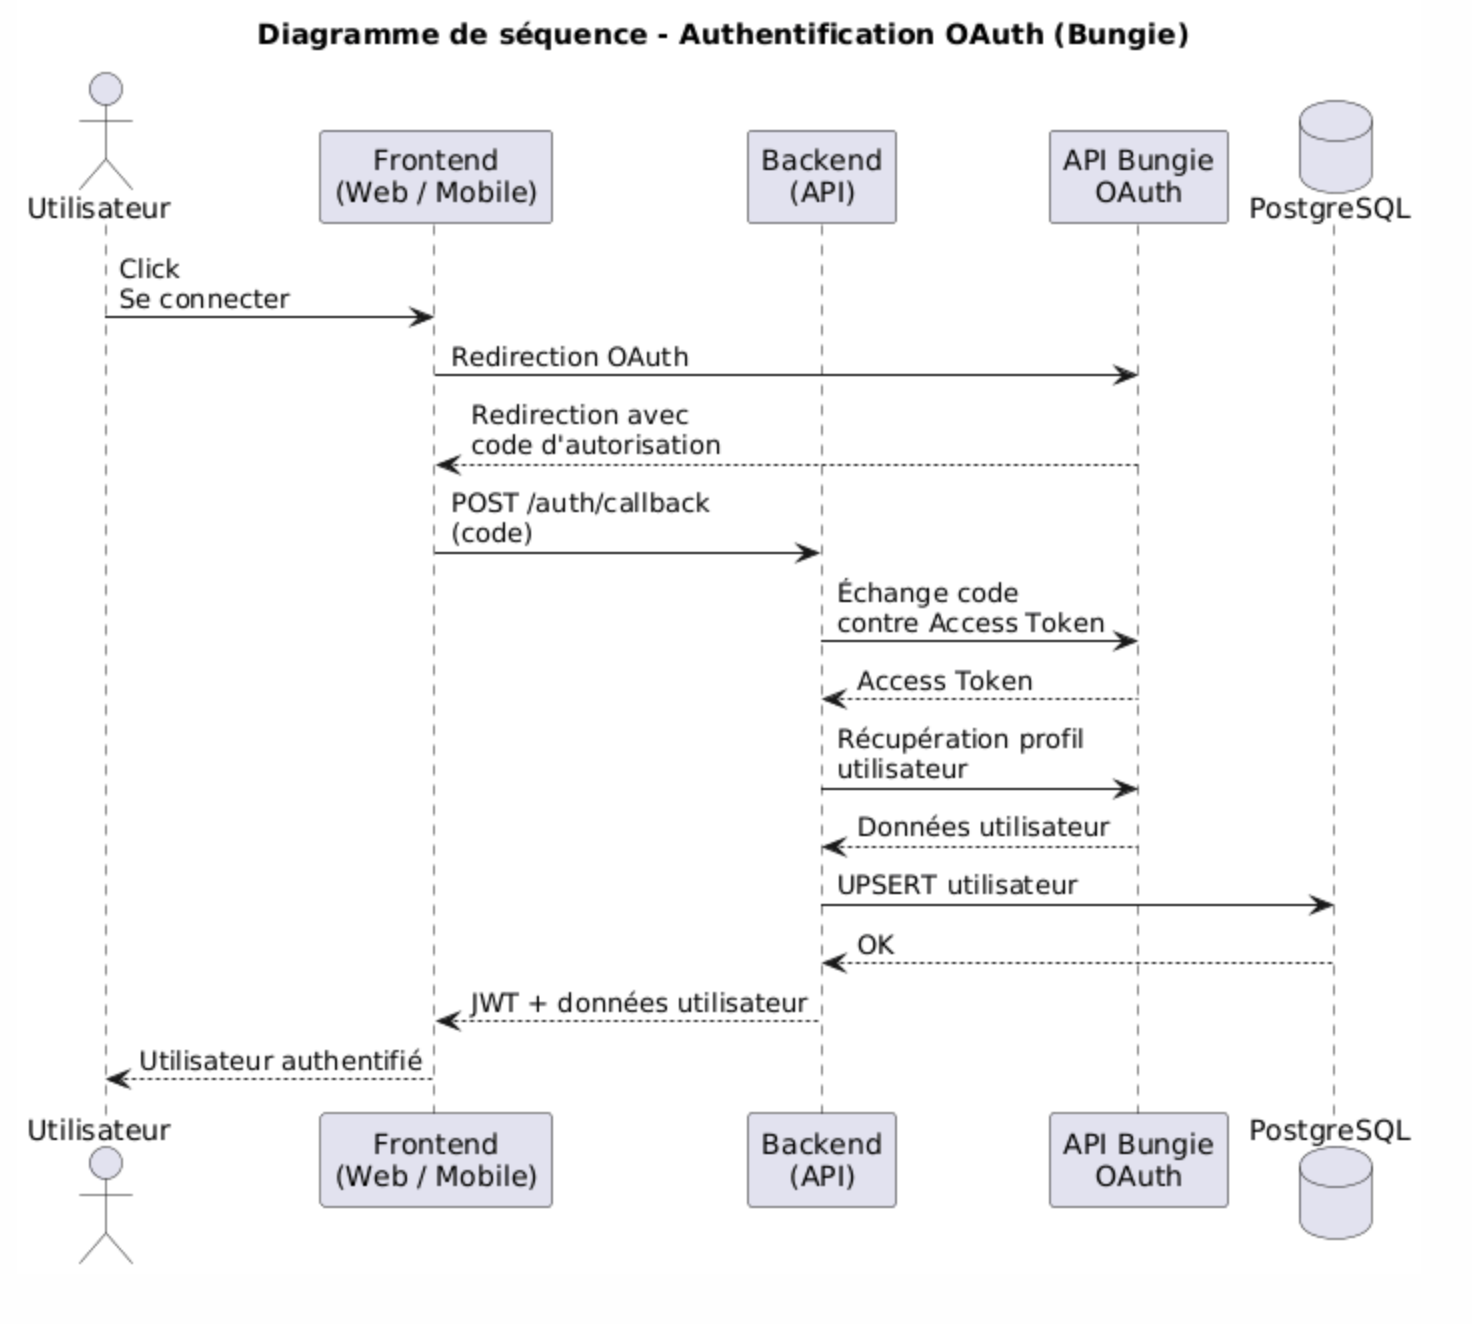
\includegraphics[width=0.8\textwidth]{assets/diagramme-seq-auth.png}
    \caption{Flux d'authentification OAuth avec Bungie}
    \label{fig:auth}
\end{figure}

\textbf{Pourquoi c'est complexe :} Il faut gérer les allers-retours avec Bungie, stocker le token de manière sécurisée, et le rafraîchir avant expiration. Si Bungie est indisponible, l'utilisateur doit avoir un message clair, pas une erreur technique.

\begin{figure}[h]
    \centering
    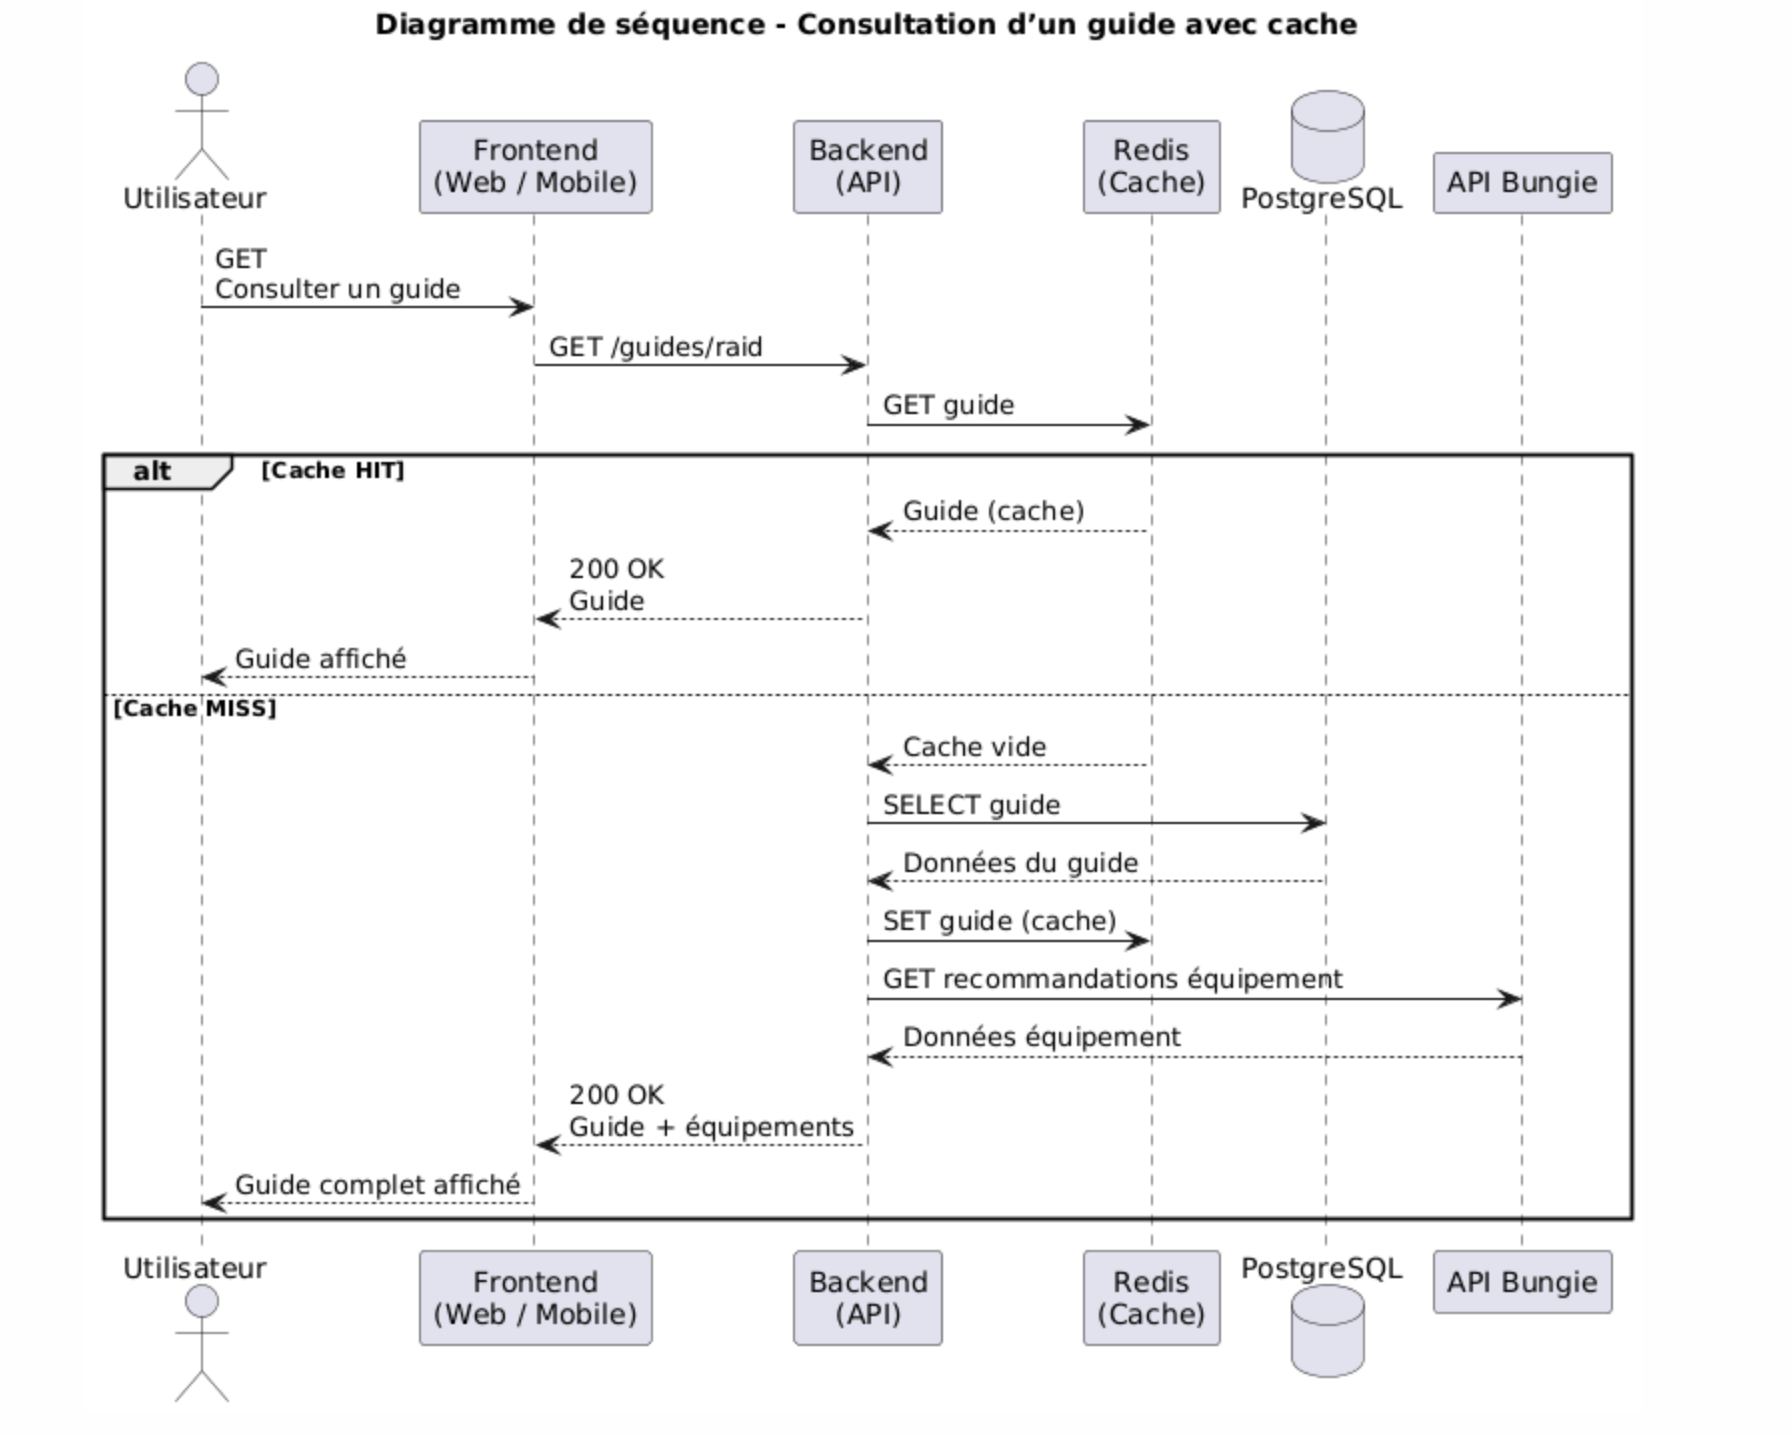
\includegraphics[width=0.8\textwidth]{assets/diagramme-seq-consult.png}
    \caption{Consultation d'un guide avec cache Redis}
    \label{fig:guide}
\end{figure}

\textbf{L'astuce technique :} Les guides sont stockés dans Redis avec une durée de vie. Si le même guide est demandé plusieurs fois, il est servi depuis le cache, ce qui est plus rapide et évite de surcharger l'API Bungie.

\section{La conception de l'interface}

\subsection{L'architecture des composants React}

J'ai organisé le frontend de manière modulaire pour faciliter la maintenance et les tests :

\begin{verbatim}
src/
├── components/
│   ├── common/        # Boutons, navigation (réutilisables)
│   ├── guides/        # Affichage des guides
│   ├── squads/        # Gestion des escouades
│   ├── calendar/      # Planification
│   └── profile/       # Profils et badges
├── hooks/              # useAuth, useSquads (logique réutilisable)
└── services/           # Appels API (Bungie, backend)
\end{verbatim}

\subsection{Exemple : le composant GuideViewer}

Ce composant illustre ma démarche de conception par composants réutilisables :
\begin{itemize}
    \item \textbf{Entrées :} identifiant du guide, callbacks de navigation
    \item \textbf{État interne :} étape en cours, progression
    \item \textbf{Optimisation :} lazy loading des images
\end{itemize}

\subsection{La charte graphique}

Inspirée de l'univers Destiny 2 :

\begin{itemize}
    \item \textbf{Couleurs :} Fond \#0A0E17 (noir bleuté), actions \#FF6B35 (orange), accents \#00E0FF (cyan)
    \item \textbf{Typographie :} Inter (lisible), tailles basées sur 2.5rem/1rem
    \item \textbf{Espacement :} Base de 8px (marges : 8, 16, 24, 32px)
\end{itemize}

\section{La conception de la base de données}

J'ai suivi la méthode Merise (MCD, MLD, MPD) pour une conception rigoureuse.

\subsection{Le Modèle Conceptuel de Données (MCD)}

\begin{figure}[h]
    \centering
    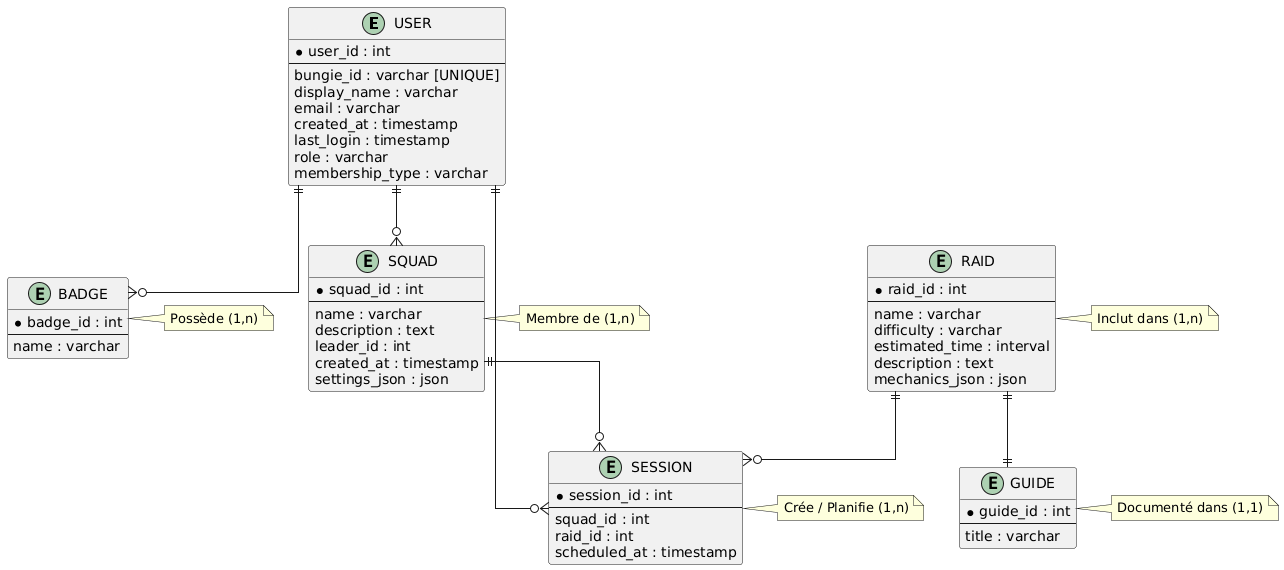
\includegraphics[width=0.8\textwidth]{assets/entite-relation.png}
    \caption{Entités : Utilisateur, Escouade, Session, Guide, Badge}
    \label{fig:mcd}
\end{figure}

\textbf{Les relations clés :}
\begin{itemize}
    \item Un \textbf{Utilisateur} peut créer plusieurs \textbf{Escouades} (en tant que leader)
    \item Un \textbf{Utilisateur} peut appartenir à plusieurs \textbf{Escouades}
    \item Une \textbf{Escouade} organise plusieurs \textbf{Sessions} de raid
\end{itemize}

\subsection{Le Modèle Physique de Données (MPD) avec Prisma}

Voici le schéma Prisma qui implémente ce modèle :

\begin{lstlisting}[language=JavaScript]
model User {
  id           Int      @id @default(autoincrement())
  bungie_id    String   @unique
  display_name String
  created_at   DateTime @default(now())
  
  squads_led   Squad[]  @relation("SquadLeader")
  squad_members SquadMember[]
  badges       UserBadge[]
}

model Squad {
  id          Int      @id @default(autoincrement())
  name        String
  leader_id   Int
  created_at  DateTime @default(now())
  max_members Int      @default(6)
  
  leader      User     @relation("SquadLeader", fields: [leader_id], references: [id])
  members     SquadMember[]
  sessions    Session[]
}

model Session {
  id           Int       @id @default(autoincrement())
  squad_id     Int
  raid_id      Int
  scheduled_at DateTime
  status       String    @default("SCHEDULED")
  
  squad        Squad     @relation(fields: [squad_id], references: [id])
}
\end{lstlisting}

\subsection{Pourquoi plusieurs bases ?}

\begin{itemize}
    \item \textbf{PostgreSQL :} Données transactionnelles (utilisateurs, escouades). Besoin de cohérence ACID.
    \item \textbf{Redis :} Cache (guides, sessions). Rapidité et expiration automatique.
    \item \textbf{MongoDB (futur) :} Logs et analytics (structure variable, volume important).
\end{itemize}

\section{L'architecture technique détaillée}

\subsection{Couche Présentation (Frontend)}

\textbf{Technologies :} React 18, Vite, TailwindCSS, React Router, Axios

L'idée est de séparer la logique d'affichage des appels API. Exemple avec le service d'authentification :

\begin{lstlisting}[language=JavaScript]
class AuthService {
  async loginWithBungie() {
    const authUrl = this.buildBungieAuthUrl();
    window.location.href = authUrl; // Redirection vers Bungie
  }
  
  async handleOAuthCallback(code) {
    const response = await api.post('/auth/callback', { code });
    this.storeTokens(response.data); // Stockage sécurisé du JWT
    return this.getUserProfile();
  }
}
\end{lstlisting}

\subsection{Couche Métier (Backend)}

\textbf{Organisation :} Contrôleurs → Services → Repositories

Cette séparation garantit que chaque composant a une responsabilité unique et facilite les tests.

\begin{lstlisting}[language=JavaScript]
// Le service contient la logique métier
class SquadService {
  async createSquad(squadData, leaderId) {
    // Règles métier : pas plus de 12 membres, max 5 escouades par joueur
    if (squadData.maxMembers > 12) {
      throw new BusinessError('Maximum 12 membres');
    }
    
    const userSquadCount = await this.squadRepository.countByUser(leaderId);
    if (userSquadCount >= 5) {
      throw new BusinessError('Limite de 5 escouades atteinte');
    }

    // Transaction pour garantir l'intégrité des données
    return await this.db.transaction(async (trx) => {
      const squad = await this.squadRepository.create(trx, {
        ...squadData,
        leader_id: leaderId
      });
      
      // Ajout automatique du leader comme membre
      await this.squadMemberRepository.create(trx, {
        squad_id: squad.id,
        user_id: leaderId,
        role: 'leader'
      });
      
      return squad;
    });
  }
}
\end{lstlisting}

\textbf{Pourquoi cette organisation ?} Elle rend le code testable et maintenable. Je peux modifier la règle des 5 escouades sans impacter le contrôleur ou le repository.

\subsection{Couche Données}

\textbf{Optimisations PostgreSQL :}
\begin{lstlisting}[language=SQL]
ALTER SYSTEM SET shared_buffers = '1GB';  -- Plus de cache
ALTER SYSTEM SET work_mem = '64MB';      -- Plus de mémoire pour les tris
\end{lstlisting}

\textbf{Stratégie Redis :}
\begin{itemize}
    \item Guides : cache 1 heure
    \item Sessions utilisateur : 24 heures
    \item Rate limiting : compteurs 15 minutes
\end{itemize}

\section{Ma stratégie de tests}

Je suis la pyramide des tests : nombreux tests unitaires, moins de tests d'intégration, encore moins d'E2E.

\subsection{Objectifs de couverture}
\begin{itemize}
    \item Unitaires : > 80\% (Jest)
    \item Intégration : > 70\% (Supertest)
    \item E2E : parcours critiques (Cypress)
\end{itemize}

\subsection{Exemple : test du service SquadService}

\begin{lstlisting}[language=JavaScript]
describe('SquadService', () => {
  it('devrait créer une escouade si les données sont valides', async () => {
    // Simulation du repository (mock)
    userRepository.getUserSquadCount.mockResolvedValue(2);
    
    const result = await squadService.createSquad(
      { name: 'Test Squad', maxMembers: 6 },
      1 // leaderId
    );
    
    expect(result).toHaveProperty('id');
    expect(result.name).toBe('Test Squad');
  });

  it('devrait refuser si limite dépassée', async () => {
    userRepository.getUserSquadCount.mockResolvedValue(5); // Déjà au max
    
    await expect(
      squadService.createSquad({ name: 'Test' }, 1)
    ).rejects.toThrow('Limite de 5 escouades atteinte');
  });
});
\end{lstlisting}

\section{Le déploiement}

\subsection{Environnements}
\begin{itemize}
    \item \textbf{Development :} local, Docker Compose
    \item \textbf{Staging :} serveur de test, identique à la prod
    \item \textbf{Production :} accessible aux utilisateurs
\end{itemize}

\subsection{Docker Compose}

\begin{lstlisting}[language=yaml]
services:
  frontend:
    build: ./frontend
    ports: ["3000:3000"]
    
  backend:
    build: ./backend
    ports: ["4000:4000"]
    environment:
      - DATABASE_URL=postgresql://user:pass@db:5432/raidcompanion
      - BUNGIE_API_KEY=${BUNGIE_API_KEY}
    depends_on:
      - db
      - redis
\end{lstlisting}

\subsection{CI/CD et monitoring}

\textbf{Pipeline :} push → tests → build image → déploiement staging → validation → production

\textbf{Surveillance :} temps de réponse, taux d'erreur, CPU, mémoire. Alertes Slack si anomalie.

\section{Ce que je retire de cette conception}

Cette approche modulaire m'a permis de :
\begin{itemize}
    \item Travailler par itérations sans tout casser
    \item Tester chaque composant isolément
    \item Préparer l'évolutivité future (ajout de MongoDB, WebSocket...)
\end{itemize}

\section{Maquettes et wireframes}

\subsection{Zoning (architecture des pages)}

\begin{figure}[h]
    \centering
    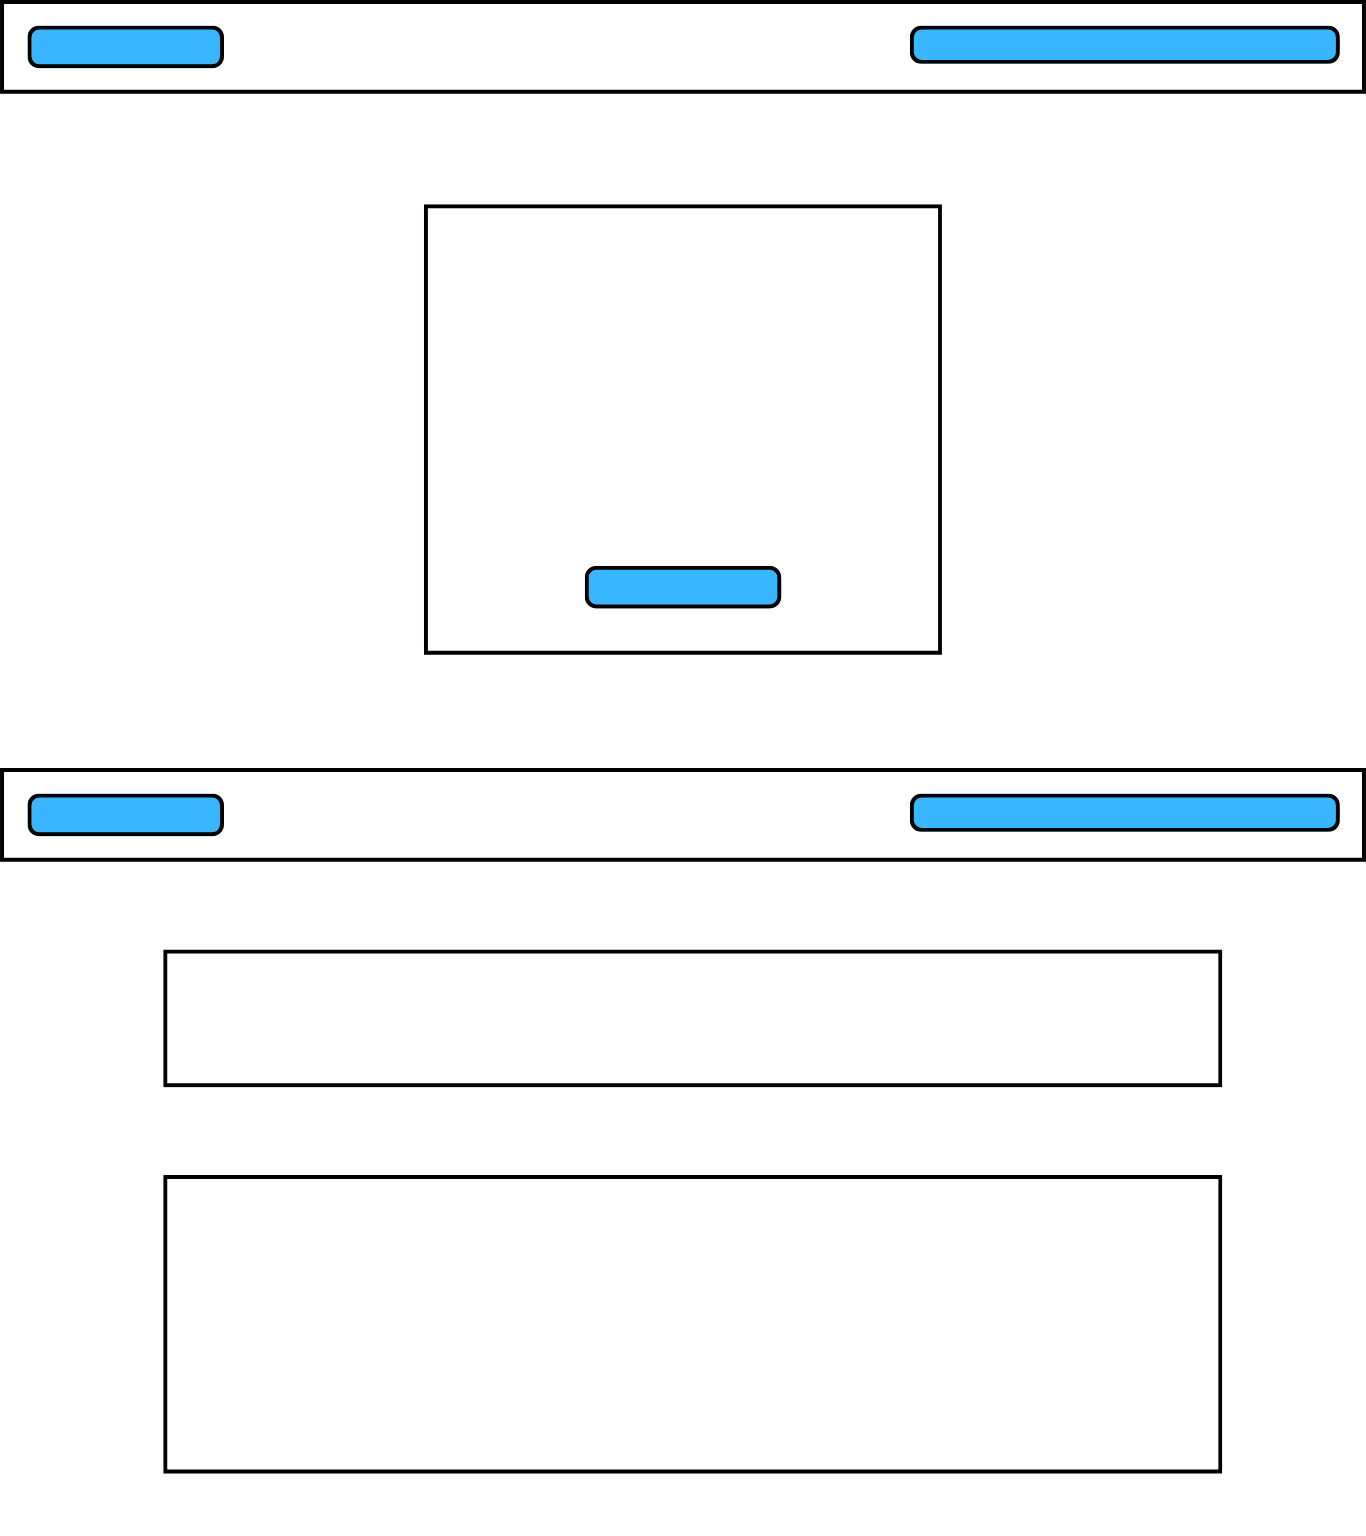
\includegraphics[width=0.3\textwidth]{assets/zoning.png}
    \caption{Zoning des pages profil et connexion}
    \label{fig:zoning}
\end{figure}

\subsection{Wireframes (maquettes basse fidélité)}

\begin{figure}[h]
    \centering
    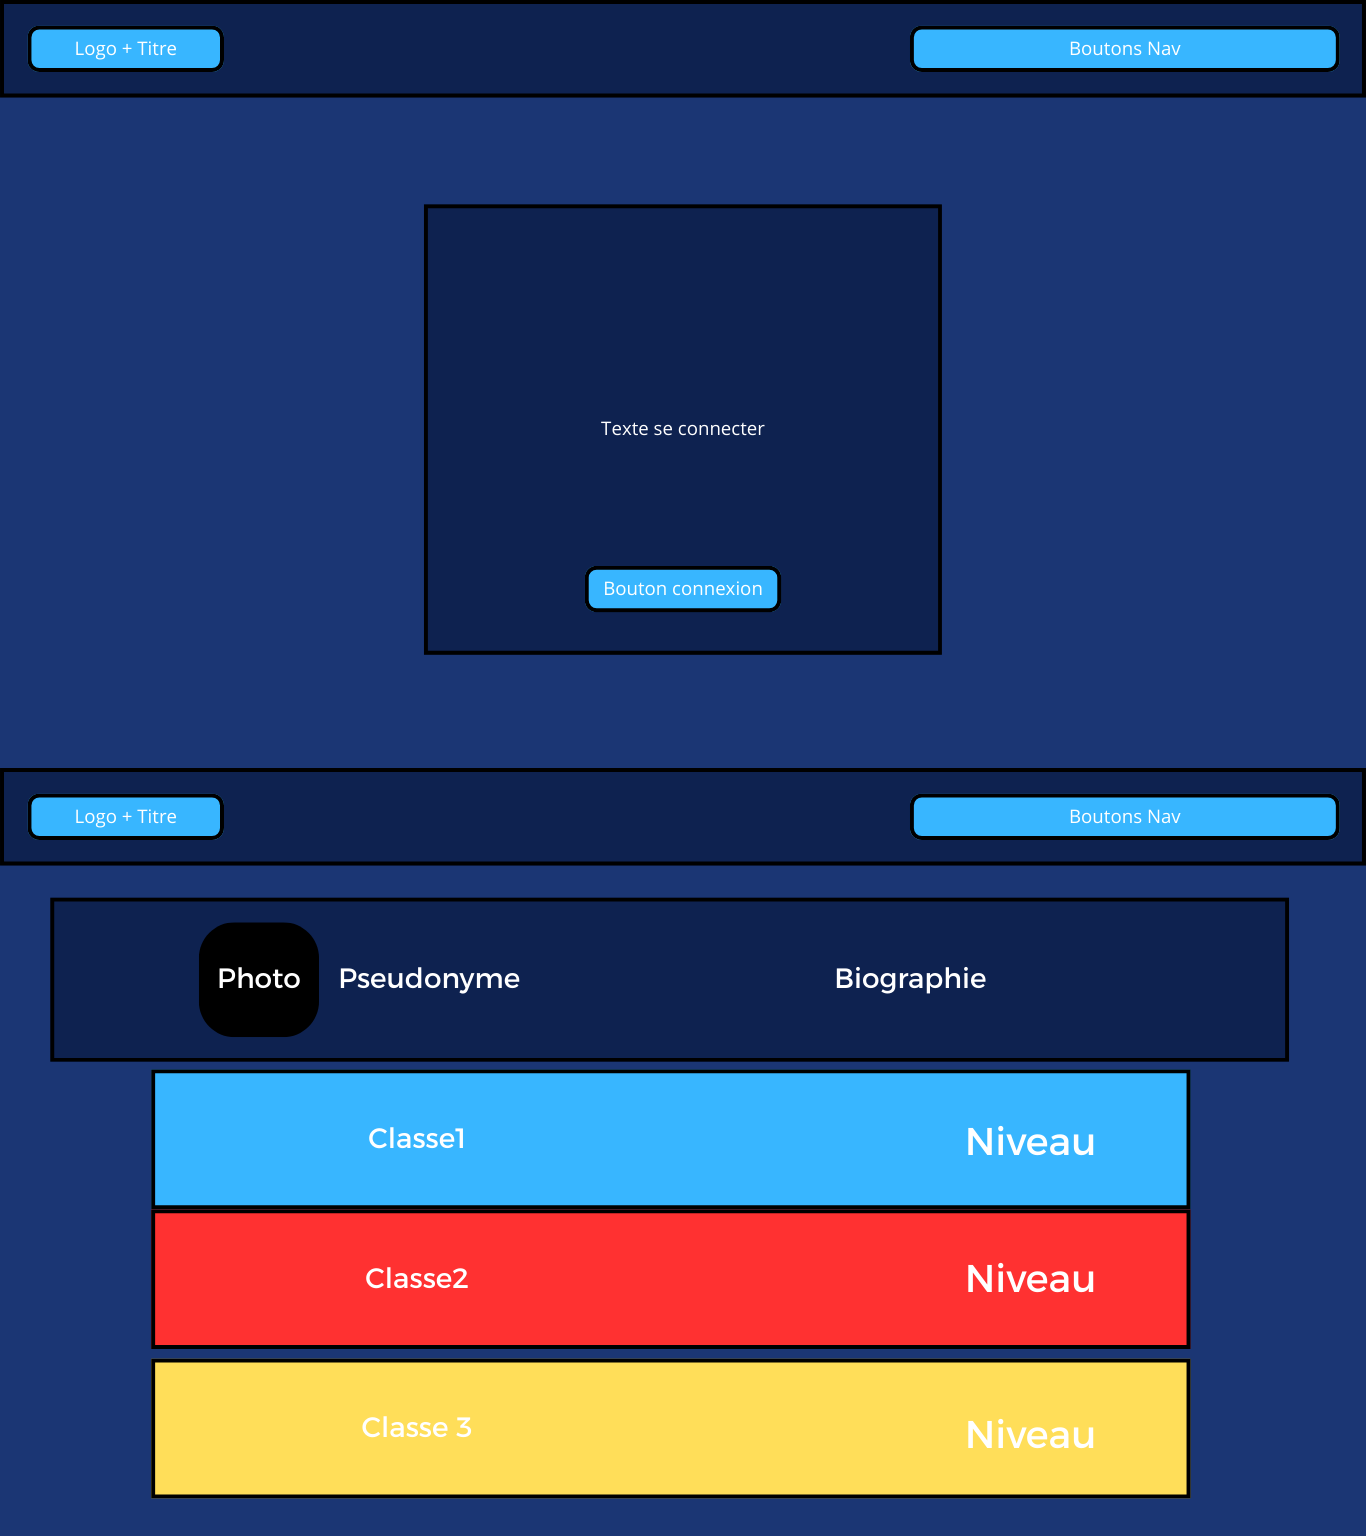
\includegraphics[width=0.3\textwidth]{assets/wireframe.png}
    \caption{Wireframe des pages profil et connexion}
    \label{fig:wireframe}
\end{figure}

\subsection{Maquettes haute fidélité}

\begin{figure}[h]
    \centering
    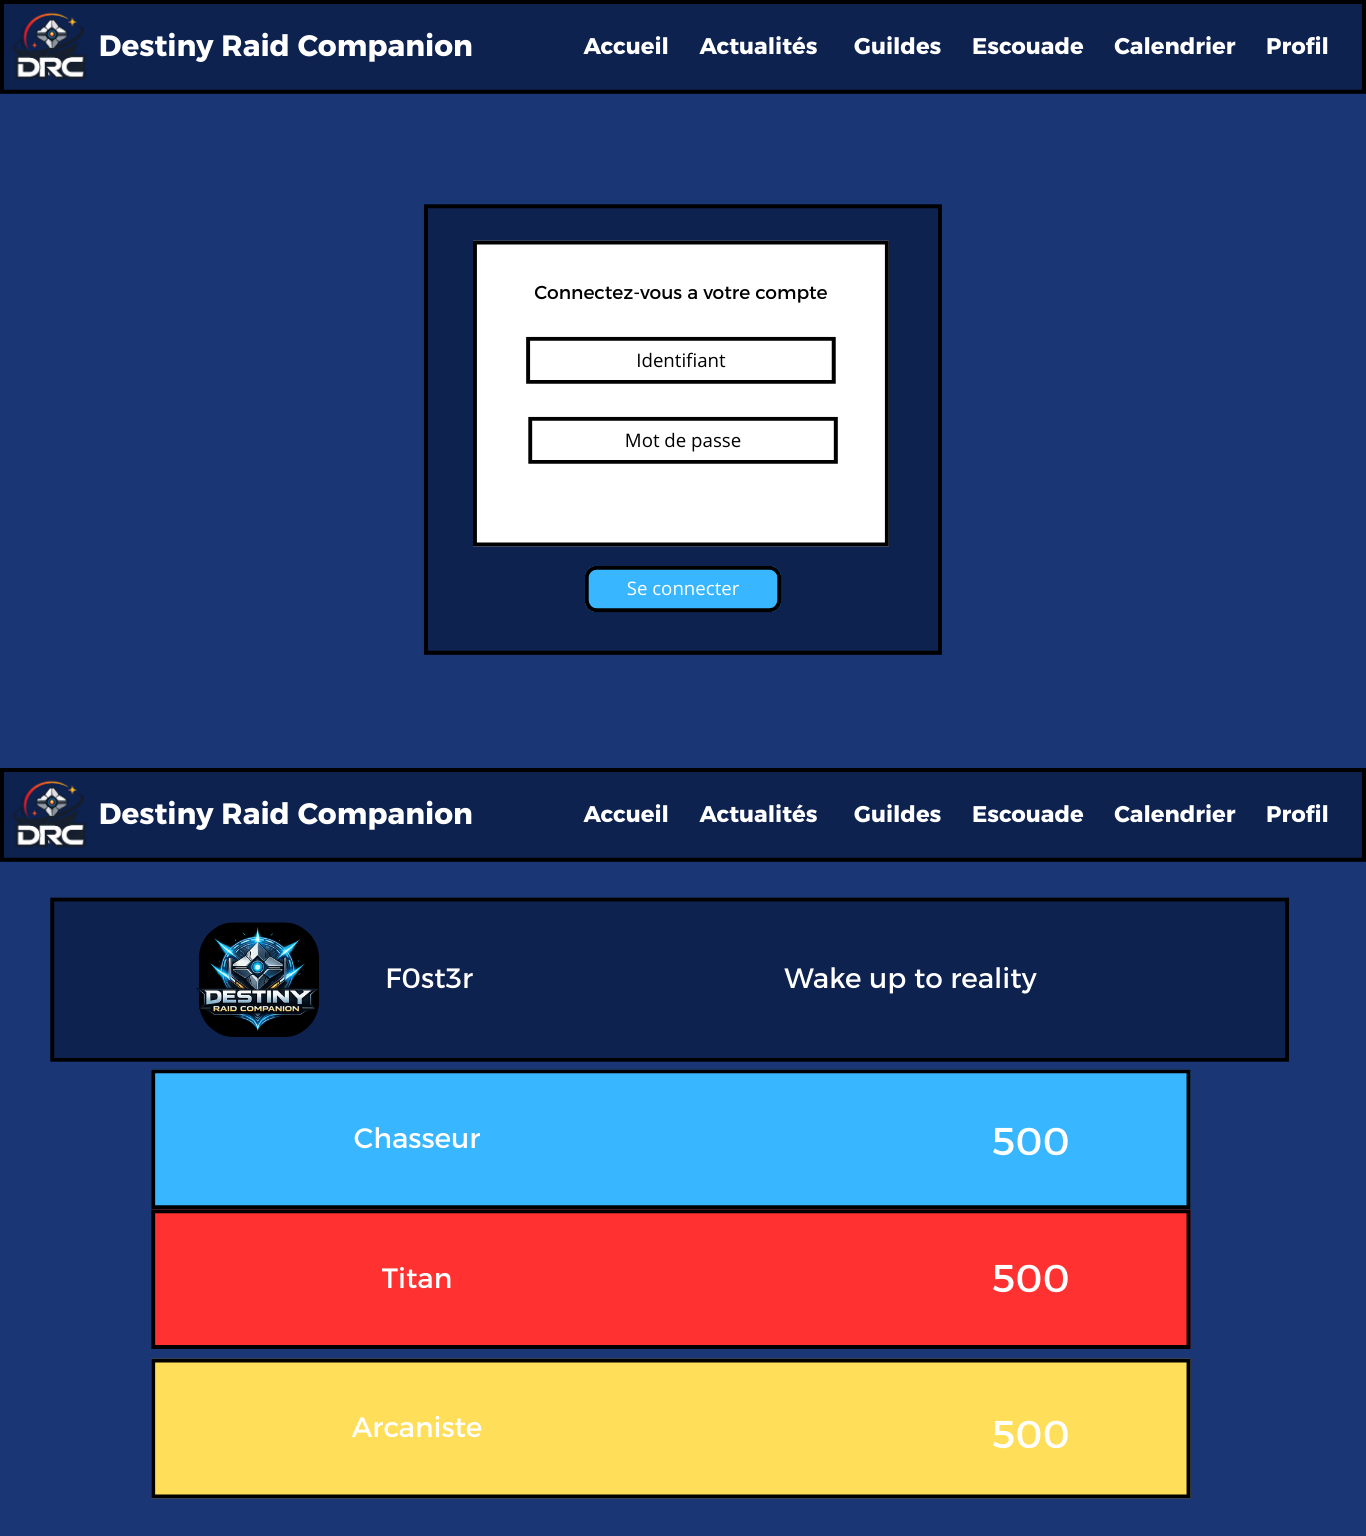
\includegraphics[width=0.3\textwidth]{assets/maquette.png}
    \caption{Maquette des pages profil et connexion}
    \label{fig:maquette}
\end{figure}

\section{Liens utiles}

\begin{itemize}
    \item React: \url{https://react.dev/}
    \item Prisma: \url{https://www.prisma.io/docs/}
    \item Docker: \url{https://docs.docker.com/}
    \item Bungie API: \url{https://bungie-net.github.io/}
\end{itemize}